%%%% fs-run-mapreduce Optimistic collision management
\label {fs-collision}

Deterministic execution is a desired property of any distributed system. 

To restrict outputs to only one possible result, we impose the following  restrictions on our model: 

\begin{itemize}
  \item We require map function to be pure: return value is only determined by its input values, without observable side effects
  \item We impose a strict ordering requirement on the grouping  input
\end{itemize}

While the former can be satisfied by moderating the  business logic, the latter is foreign to the distributed systems: 
it is hard to ensure the right order of delivery due to asynchrony inherent for a distributed system. There are two most common methods that are used to implement order-sensitive operators: in-order processing (IOP)~\cite{Arasu:2006:CCQ:1146461.1146463, Cranor:2003:GSD:872757.872838} and out-of-order processing (OOP)~\cite{Li:2008:OPN:1453856.1453890}. According to IOP approach, each operation must enforce the total order on output elements. This method does not scale well, because it requires buffering before each, even stateless, operation within pipeline until the total order is reached~\cite{Li:2008:OPN:1453856.1453890}. OOP is an approach that does not require order maintenance if it is not needed. In the case of ordering requirements, OOP buffers input items until a special condition is satisfied. This condition is based on progress indicators such as punctuations~\cite{Tucker:2003:EPS:776752.776780}, low watermarks~\cite{Akidau:2013:MFS:2536222.2536229}, or heartbeats~\cite{Srivastava:2004:FTM:1055558.1055596}.  

Some state-of-the-art stream processing systems adopt OOP~\cite{Carbone:2017:SMA:3137765.3137777}, but they suppose that items must be buffered before each order-sensitive operation, if deterministic results are required. In our system, we use an optimistic approach for handling out-of-order items, that is based on OOP, but require single buffer per computational pipeline, no matter how many stateful operations it contains.
%
% \subsection{Optimistic approach}
%
%As it was defined previously, 

Only the grouping operation retains a dependency on the order of incoming items. 
%Therefore, there is a need to enforce the right order to achieve deterministic processing.
%
%As it was mentioned above, conservative methods for order enforcing can imply high latency overhead. 
Within the  optimistic approach, we accept the fact that grouping can produce incorrect output, but we guarantee that all correct groups are eventually produced. 
%The correctness of tuple means that this tuple would be generated if the order assumption was satisfied.
To eventually produce all correct tuples, we use an approach called {\it repair}. 
If an item preceeing already processed items arrives at the grouping operation, all items starting with the just arrived one are re-processed, and {\em tombstones} (invalidator) are generated for all items produced earlier for all input items processed before the new one. A tombstone for an item is the same item marked with a flag in its meta-information. Hence, it traverses over the same physical path as the invalidated item.

An example of grouping repair is shown in Figure~\ref{grouping-replaying}, 
The green item is out-of-order. 
The output consists of the new valid items  $(1, 2)$ and $(2, 3)$  and the tombstone $(1, 3)_tomb$ for the previously generated item.

\begin{figure}[ht]
  \centering
  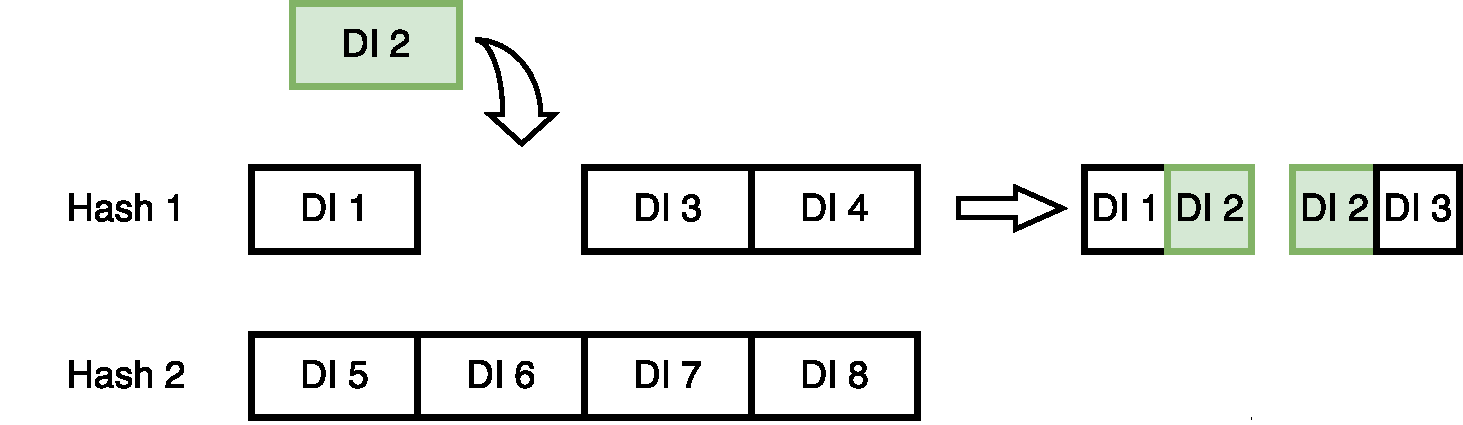
\includegraphics[width=0.6\textwidth]{pics/grouping-replaying}
  \caption{The repair in grouping with $WindowSize = 2$. % New items are generated on insertion
  }
  \label {grouping-replaying}
\end{figure}

%In the case of the right order of input items, there are no redundant items produced.

The barrier  keeps outgoing items on hold and filters out invalid elements, when corresponding tombstones arrive. 
As soon as no tombstones preceding certain point cannot arrive any more, items are delivered  up to this point. 
%
%It is partially flushed for some meta-information interval when there is a guarantee that there are no any out-of-order items and tombstones further up the stream for this range.
More details can be found  in section~\ref{fs-impl}.

% \subsection{Advantages and limitations}

%The proposed architecture's performance depends on how often reorderings are observed during the runtime. In the case when the order naturally preserved there is almost no overhead: when the watermark arrives, all computations are already done. 
%The probability of reordering could be managed on a business-logic level and optimized by the developer. In experiments section it is shown that the computational nodes count is one of such parameters. Regarding the weaknesses, this method can generate additional items, which lead to extra network traffic and computations. Experiments, which are shown in the section~\ref{fs-experiments-section} demonstrate that the number of extra items is low.

